%\documentclass[a4paper,11pt]{book}
\documentclass[a4paper,twoside,10pt,titlepage]{book}
\usepackage{listings}
\usepackage[utf8]{inputenc}
\usepackage[spanish]{babel}

\usepackage{xspace}

\decimalpoint
\usepackage{dcolumn}
\newcolumntype{.}{D{.}{\esperiod}{-1}}
\makeatletter
\addto\shorthandsspanish{\let\esperiod\es@period@code}
\makeatother


%\usepackage[chapter]{algorithm}
\RequirePackage{verbatim}
%\RequirePackage[Glenn]{fncychap}
\usepackage{fancyhdr}
\usepackage{graphicx}
\usepackage{afterpage}
\usepackage{longtable}
\usepackage{natbib}
\usepackage{float}


% ********************************************************************
% Re-usable information
% ********************************************************************
%\newcommand{\myTitle}{FPGAs de Xilinx \xspace}
\newcommand{\myTitle}{Plataforma didáctica para desarrollo de sistemas basados en FPGAs de Xilinx}
\newcommand{\myDegree}{Grado en Ingeniería Informática\xspace}
\newcommand{\myName}{Elena Cantero Molina alumna\xspace}
\newcommand{\myProf}{María Begoña del Pino Prieto tutora\xspace}
%\newcommand{\mySupervisor}{Put name here\xspace}
\newcommand{\myFaculty}{Escuela Técnica Superior de Ingenierías Informática y de Telecomunicación\xspace}
\newcommand{\myFacultyShort}{E.T.S. de Ingenierías Informática y de
Telecomunicación\xspace}
%\newcommand{\myDepartment}{Departamento de ...\xspace}
\newcommand{\myUni}{\protect{Universidad de Granada}\xspace}
\newcommand{\myLocation}{Granada\xspace}
\newcommand{\myTime}{\today\xspace}
\newcommand{\myVersion}{Version 0.1\xspace}

\usepackage{url}
\usepackage{colortbl,longtable}
\usepackage[stable]{footmisc}
%\usepackage{index}

\pagestyle{fancy}
\fancyhf{}
\fancyhead[LO]{\leftmark}
\fancyhead[RE]{\rightmark}
\fancyhead[RO,LE]{\textbf{\thepage}}
\renewcommand{\chaptermark}[1]{\markboth{\textbf{#1}}{}}
\renewcommand{\sectionmark}[1]{\markright{\textbf{\thesection. #1}}}

\setlength{\headheight}{1.5\headheight}

\newcommand{\HRule}{\rule{\linewidth}{0.5mm}}

\definecolor{gray97}{gray}{.97}
\definecolor{gray75}{gray}{.75}
\definecolor{gray45}{gray}{.45}
\definecolor{gray30}{gray}{.94}

\lstset{ frame=Ltb,
     framerule=0.5pt,
     aboveskip=0.5cm,
     framextopmargin=3pt,
     framexbottommargin=3pt,
     framexleftmargin=0.1cm,
     framesep=0pt,
     rulesep=.4pt,
     backgroundcolor=\color{gray97},
     rulesepcolor=\color{black},
     %
     stringstyle=\ttfamily,
     showstringspaces = false,
     basicstyle=\scriptsize\ttfamily,
     commentstyle=\color{gray45},
     keywordstyle=\bfseries,
     %
     numbers=left,
     numbersep=6pt,
     numberstyle=\tiny,
     numberfirstline = false,
     breaklines=true,
   }
 
% minimizar fragmentado de listados
\lstnewenvironment{listing}[1][]
   {\lstset{#1}\pagebreak[0]}{\pagebreak[0]}

 
\lstdefinestyle{Consola}
   {basicstyle=\scriptsize\bf\ttfamily,
    backgroundcolor=\color{gray30},
    frame=single,
    numbers=none
   }


\newcommand{\bigrule}{\titlerule[0.5mm]}


%Para conseguir que en las páginas en blanco no ponga cabecerass
\makeatletter
\def\clearpage{%
  \ifvmode
    \ifnum \@dbltopnum =\m@ne
      \ifdim \pagetotal <\topskip
        \hbox{}
      \fi
    \fi
  \fi
  \newpage
  \thispagestyle{empty}
  \write\m@ne{}
  \vbox{}
  \penalty -\@Mi
}
\makeatother

\usepackage{pdfpages}
\begin{document}
\begin{titlepage}
 
 
\newlength{\centeroffset}
\setlength{\centeroffset}{-0.5\oddsidemargin}
\addtolength{\centeroffset}{0.5\evensidemargin}
\thispagestyle{empty}

\noindent\hspace*{\centeroffset}\begin{minipage}{\textwidth}

\centering
\includegraphics[width=0.9\textwidth]{imagenes/logo_ugr.jpg}\\[1.4cm]

\textsc{ \Large TRABAJO FIN DE GRADO\\[0.2cm]}
\textsc{ INGENIERÍA EN INGENIERÍA INFORMÁTICA}\\[1cm]
% Upper part of the page
% 
% Title
{\Huge\bfseries \myTitle}
\noindent\rule[-1ex]{\textwidth}{3pt}\\[3.5ex]
{\large\bfseries \mySubTitle}
\end{minipage}

\vspace{2.5cm}
\noindent\hspace*{\centeroffset}\begin{minipage}{\textwidth}
\centering

\textbf{Autora}\\ {\myName}\\[2.5ex]
\textbf{Directora}\\
{\myProf}\\[2cm]
\includegraphics[width=0.3\textwidth]{imagenes/etsiit_logo.png}\\[0.1cm]
\textsc{\myFaculty}\\
\textsc{---}\\
\textsc{\myLocation, \myTime}
\end{minipage}
%\addtolength{\textwidth}{\centeroffset}
%\vspace{\stretch{2}}
\end{titlepage}



%%\thispagestyle{empty}
%\cleardoublepage

\thispagestyle{empty}

\begin{center}
{\large\bfseries Título del Proyecto: \mySubTitle}\\
\end{center}
\begin{center}
\myName\\
\end{center}

Introducción y/o presentación

%\vspace{0.7cm}
\noindent{\textbf{Palabras clave}: palabra\_clave1, palabra\_clave2, palabra\_clave3, ......}\\

\vspace{0.7cm}
\noindent{\textbf{Resumen}}\\

Poner aquí el resumen.
\cleardoublepage


\thispagestyle{empty}


\begin{center}
{\large\bfseries Project Title: Project Subtitle}\\
\end{center}
\begin{center}
First name, Family name (student)\\
\end{center}

%\vspace{0.7cm}
\noindent{\textbf{Keywords}: Keyword1, Keyword2, Keyword3, ....}\\

\vspace{0.7cm}
\noindent{\textbf{Abstract}}\\

Write here the abstract in English.

\clearpage
\thispagestyle{empty}

\noindent\rule[-1ex]{\textwidth}{2pt}\\[4.5ex]

Yo, \textbf{Elena Cantero Molina}, alumna de la titulación \myDegree de la \textbf{Escuela Técnica Superior
de Ingenierías Informática y de Telecomunicación de la Universidad de Granada}, con DNI 45744912M, autorizo la
ubicación de la siguiente copia de mi Trabajo Fin de Grado en la biblioteca del centro para que pueda ser
consultada por las personas que lo deseen.

\vspace{6cm}

\noindent Fdo: Elena Cantero Molina

\vspace{2cm}

\begin{flushright}
Granada a X de mes de 2020.
\end{flushright}

\clearpage
\thispagestyle{empty}

\noindent\rule[-1ex]{\textwidth}{2pt}\\[4.5ex]

D. \textbf{\myProf}, Profesor del Área de XXXX del Departamento YYYY de la Universidad de Granada.

\vspace{0.5cm}

\textbf{Informa:}

\vspace{0.5cm}

Que el presente trabajo, titulado \textit{\textbf{\myTitle, \mySubTitle}},
ha sido realizado bajo su supervisión por \textbf{\myName}, y autorizamos la defensa de dicho trabajo ante el tribunal
que corresponda.

\vspace{0.5cm}

Y para que conste, expiden y firman el presente informe en Granada a X de mes de 2020.

\vspace{1cm}

\textbf{La directora:}

\vspace{5cm}

\noindent \textbf{\myProf}

\chapter*{Agradecimientos}
\thispagestyle{empty}

       \vspace{1cm}


Poner aquí agradecimientos...


\frontmatter
\tableofcontents
\listoffigures
%\listoftables
%
\mainmatter
\setlength{\parskip}{5pt}

En este trabajo de fin de grado se ha realizado un estudio de una plataforma didáctica para desarrollo de sistemas basados en FPGAs de Xilinx. 
Una \textbf{FPGA} es un dispositivo semiconductor basado en matrices de bloques lógicos configurables que están conectados mediante interconexiones programables. 
Para programarlas existen tres principales tecnologías, la tecnología Antifusible que no es reprogramable, la tecnología SRAM que es reprogramable 
pero con memoria volátil y la tecnología Flash que es reprogramable pero con memoria no volátil. 

Actualmente las FPGAs pueden ser usadas para implementar sistemas en distintos ámbitos, como por ejemplo Aeroespacial y defensa, 
Centro de procesamiento de datos, Industria, Medicina o Comunicaciones.

Dentro de los principales fabricantes de FPGAs, destaca \textbf{Xilinx} como el principal fabricante, seguido de Intel. Las características de sus dispositivos 
y herramientas sofwtare de desarrollo son descritas en esta memoria.

La tarjeta que se va a usar en este proyecto para el desarrollo del mismo es la tarjeta \textbf{ZYBO} que incluye una FPGA de la familia Zynq-7000 de Xilinx. Esta FPGA incluye 
un sistema de procesamiento basado en cores ARM empotrados, memoria ``on-chip'', interfaces de memoria externa y lógica genérica basada en tecnología SRAM. La arquitectura 
de esta FPGA permite la implementación de lógica personalizada para configurar módulos hardware específicos y la ejecución de software en los procesadores empotrados, los cuales 
son explicados en el desarrollo de la memoria. 

Xilinx ha sido una empresa pionera en la comercialización de herramientas de síntesis de alto nivel para describir componentes hardware a partir de descripciones C/C++ 
con el módulo Vivado HLS que se ha utilizado en asignaturas de perfil avanzado. En este trabajo se plantea la migración a Vivado de prácticas de laboratorio 
de un asignatura de carácter más básico donde se estudia el diseño de componentes a partir de herramientas de síntesis RT-lógica en las que se utilizan lenguajes 
de descripción hardware tipo \textbf{VHDL} o \textbf{Verilog}. El lenguaje usado en este trabajo es VHDL.

El objetivo de este trabajo es conocer la plataforma \textbf{Vivado} y realizar un flujo de diseño apoyándonos en la propia tarjeta. Vivado está preparado 
para la síntesis y análisis de diseños HDL. Para ello, hay que conocer las posibilidades que tiene Vivado para cada fase del flujo de diseño. Así, se ha estudiado cómo 
se implementan las diferentes fases del flujo de diseño con esta herramienta. A continuación, se ha realizado una descripción de los principales módulos que se van a 
usar en la posterior realización de casos prácticos. Estos módulos son los más relevantes para la finalidad de este proyecto, existiendo muchos más. En concreto son, 
un procesador didáctico, una memoria RAM, un módulo generador de reloj y un controlador VGA.

Después, como casos prácticos se detallan un computador básico, en el que se usa el bloque de memoria RAM, y la visualización en pantalla de una bola moviéndose 
en ella, en el que se usa el módulo generador de reloj y el controlador VGA.

Por último se realiza la conclusión final del trabajo, donde se muestra si se han conseguido los objetivos planteados y además se incluyen otras vías futuras que se 
pueden realizar a partir de este proyecto.

\chapter{Resumen extendido y palabras clave en inglés}



\chapter{Motivación e introducción}


\section{Sistemas basados en dispositivos FPGAs} 

Las FPGAs (\textit{Field Programmable Gate Arrays}), son dispositivos semiconductores basados en matrices de bloques lógicos configurables
(\textbf{CLB}) que están conectados mediante interconexiones programables \cite{fpga_xilinx}. 

Los bloques lógicos configurables en las FPGAs basadas en celdas SRAM incluyen LUTs (\textit{tablas de consulta}), flip-flops y 
multiplexores de entrada y salida (Figura \ref{arqFPGA}). Una LUT almacena una lista de salidas lógicas para cualquier combinación de 
entradas.

\begin{figure}[H]
    \centering
    \includegraphics[width = 0.5\textwidth]{imagenes/arqFPGA.png}
    \caption{\textit{Arquitectura de una FPGA}}\label{arqFPGA}
\end{figure}

Estas FPGAs pueden ser reprogramadas para  algún trabajo específico o para cambiar los requisitos de funcionalidad después de su 
fabricación. Algunas pueden ser programadas una sola vez mientras que otras pueden ser reprogramadas una y otra vez. A estos 
dispositivos que son programados una única vez son referidos como \textbf{OTP} (\textit{one-time programmable}).

\textit{Field Programmable}, se refiere al hecho de que su programación se hace ``\textit{en el campo}'' a diferencia de otros dispositivos 
que su funcionalidad está programada por el fabricante \cite{maxfield1}.

Las tres principales tecnologías usadas para programar una FPGA son: \textbf{Antifusible}, \textbf{SRAM}, \textbf{Flash}

La tecnología \textbf{Antifusible} es una tecnología no reprogramable, por lo tanto son \textit{OTP}. Son dispositivos que permiten establecer 
conexiones entre distintas capas de metal. No es volátil y además la conexión entre los bloques lógicos tiene un retardo muy reducido, por lo 
que el rendimiento es alto. Sin embargo, las FPGAs antifusibles necesitan un proceso de fabricación específico y por lo tanto es caro. 

La tecnología \textbf{SRAM} es una tecnología reprogramable con una reprogramación muy rápida. Sin embargo, las FPGAs basadas en esta tecnología 
con volátiles, lo que significa que los datos de configuración del dispositivo se perderán cuando se desconecte la energía. 

La tecnología \textbf{Flash} es reprogramable como la \textbf{SRAM} y además es no volátil como la \textbf{Antifusible}. Utiliza menos potencia 
que la \textbf{Antifusible} con un proceso de fabricación como la \textbf{SRAM}.

Hay muchos tipos diferentes de circuitos integrados digitales, entre los que destacamos \textbf{PLDs} (\textit{Programmable Logic Devices}), 
\textbf{ASICs} (\textit{Application-Specific Integrated circuits}), \textbf{ASSPs} (\textit{Application-Specific Standard Parts}) y \textbf{FPGAs}.

Los \textbf{PLDs} son dispositivos con una arquitectura interna predeterminada por el fabricante, creados para ser configurados por 
ingenieros en el campo para realizar diferentes funciones. En comparación a las \textbf{FPGAs}, contiene un número limitado de puertas lógicas 
y las funciones que se suelen implementar son más pequeñas y simples.

Por otro lado los \textbf{ASICs} y los \textbf{ASSPs} contienen cientos de millones de puertas lógicas y se usan para crear grandes y complejas 
funciones. Ambos están basados en los mismos procesos de diseño y tecnologías y pueden ser usados por millones de usuarios y compañias. La 
única diferencia es que un \textbf{ASIC} está diseñado y fabricado para una aplicación en concreto, mientras que un \textbf{ASSP} lo está 
para un dominio de aplicaciones.

Así, las \textbf{FPGAs} se encuentran entre los \textbf{PLDs} y los \textbf{ASICs} porque su funcionalidad puede ser diseñada en el campo como 
los \textbf{PLDs}, pero pueden contener millones de puertas lógicas y ser usadas para implementar funciones complejas que previamente sólo 
podían ser realizadas usando \textbf{ASICs}. 

El coste de un diseño de \textbf{FPGA} es mucho menor que el de uno de un \textbf{ASIC}. Al mismo tiempo, los cambios de diseño implementados 
son más fáciles en \textbf{FPGAs} y el tiempo de comercialización es más rápido \cite{maxfield2}.

Las FPGAs \textbf{SoC}(\textit{System-on-chip}, que es un circuito integrado que tiene todos los componentes necesarios para un sistema electrónico.
Además de la lógica genérica configurable incluyen empotrados en hardware uno o varios procesadores, memoria DDR, interfaces para buses 
estándar, interfaces de comunicaciones, e incluso unidades de procesamiento gráfico.) tienen una gran capacidad de procesamiento para 
adaptarse a diferentes aplicaciones. Un SoC de bajo costo y consumo se puede utilizar en aplicaciones como tarjetas de procesamiento de 
vídeo. Sin embargo, hay otros SoCs que se utilizan en aplicaciones de alto rendimiento en comunicaciones o computación de alto rendimiento.

A mediados del año 1980 llegaron las FPGAs, que eran usadas para implementar lógicas simples, máquinas de estados con una complejidad media 
y tareas de procesamiento de datos. A principios de los 90s, el mercado en el que se vendían se extendió al área de las telecomunicaciones 
debido a que el tamaño y sofisticación de las mismas empezaron a crecer. A finales de los 90s, el uso de las FPGAs en aplicaciones de consumo 
e industriales tuvo un enorme crecimiento.

Las FPGAs a menudo son utilizadas para crear prototipos de diseños ASIC o para tener un plataforma hardware donde verificar la implementación 
física de nuevos algoritmos \cite{maxfield1}. 

Actualmente se pueden encontrar FPGAs de alto rendimiento con millones de puertas. Algunos de estos dispositivos tienen núcleos de 
microprocesador integrados, dispositivos de entrada-salida de alta velocidad y similares. El resultado es que actualmente las FPGAs pueden ser 
usadas para implementar casi cualquier cosa en distintos ámbitos como por ejemplo:

\begin{itemize}
    \item \textbf{Aeroespacial y defensa} 
    \item \textbf{Emulación y Prototipado}
    \item \textbf{Audio} 
    \item \textbf{Automoción} 
    \item \textbf{Broadcast} 
    \item \textbf{Electrónica de consumo} 
    \item \textbf{Centro de procesamiento de datos} 
    \item \textbf{Computación de alto rendimiento} 
    \item \textbf{Industria} 
    \item \textbf{Medicina} 
    \item \textbf{Comunicaciones}
    \item \textbf{Inteligencia Artificial}
    \item \textbf{Procesamiento de imágenes}
    \item \textbf{Seguridad}
\end{itemize}

\section{Niveles de síntesis automática}
La metodología es un concepto abstracto referido a un conjunto de procesos que relacionan entre sí los niveles de complejidad y abstracción 
(\textit{funcional o de comportamiento}, \textit{arquitectural o transferencia de registros}, \textit{lógico o de puertas} y 
\textit{físico}), por los que pasa el diseño de un circuito \cite{teres1997vhdl}.

Los niveles de abstracción son:

\begin{itemize}
    \item \textbf{Funcional o de comportamiento}: Se indica el comportamiento del circuito como una relación funcional entre las entradas 
    y salidas, sin tener en cuenta la implementación.
    \item \textbf{Arquitectural o de transferencia de resgistros}: Se realiza una partición de bloques funcionales y se planifican las 
    acciones que se vayan a hacer. 
    \item \textbf{Lógico o de puertas}: Componentes expresados como ecuaciones lógicas o puertas y elementos de una biblioteca genérica o 
    específica de una tecnología.
    \item \textbf{Físico}
\end{itemize}

En general, establecer una metodología o flujo de diseño consiste en definir las distintas etapas por los que pasarán los distintos niveles 
de abstracción y fijar cómo pasar de unos niveles de abstracción a otros usando procesos manuales o automáticos de:

\begin{itemize}
    \item \textbf{Síntesis}: Pasar descripciones de un nivel de abstracción a otro con mayor detalle (por ejemplo, de una descripción RT a 
    puertas, o de puertas a física).
    \item \textbf{Análisis}: Extraer información de un descripción para verificar prestaciones o para validar restricciones en un nivel 
    de abstracción superior.
    \item \textbf{Verificación / Simulación}: Validar las descripciones de cada etapa.
\end{itemize}

Para la realización del flujo de diseño, se puede seguir una evolución ``\textit{Top-Down}'' empezando por la idea de la implementación 
o se puede seguir una evolución ``\textit{Bottom-Up}'' comenzando por el nivel físico hasta llegar al funcional.

El diseño ``\textit{Top-Down}'' consiste en coger una idea con un alto nivel de abstracción y partiendo de ella, implementarla y si es necesario 
incrementar el nivel de detalle. Con este diseño se consigue una mayor adecuación a las especificaciones y requisitos.

El diseño ``\textit{Bottom-Up}'' consiste en la descripción del circuito con componentes que se pueden agrupar en módulos hasta llegar al 
sistema completo que se desea. Este diseño está condicionado por los componentes del diseño que están disponibles.

PONER LO DE LOS LENGUAJES VHDL Y VERILOG--------------------------------------------------------------------------

Una de las características principales de un lenguaje de descripción hardware es que a partir de una descripción se puede generar un 
circuito físico. La síntesis es el paso de un nivel de descripción a uno de nivel inferior.

La síntesis física consiste en la ubicación, es decir, decidir dónde colocar todos elementos lógicos, y en el enrutamiento, en el que se 
decide cómo se interconectan los elementos en la FPGA.

La síntesis RT-lógica es un proceso en el se crea un diseño RTL (\textit{Register-Transfer Level}), que es una abstracción del diseño 
en el que se modela el circuito digital, y luego esa representación RTL es convertida a un conjunto de registros y ecuaciones 
booleanas equivalentes. 

La principal diferencia entre síntesis RT y síntesis de alto nivel es que la primera parte de una descripción en la que de forma 
explícita se especifican las operaciones que deben realizarse en cada ciclo de reloj, mientras que la planificación de operaciones 
en ciclos de reloj se realiza de forma automática en la segunda.

La síntesis de alto nivel une hardware y software de manera que los diseñadores hardware pueden trabajar con un alto nivel de abstracción 
y los desarrolladores software pueden acelerar partes computacionalmente complejas de sus algoritmos en una FPGA. 

El uso de una metodología de diseño de síntesis de alto nivel permite desarrollar algoritmos con respecto a la implementación ya que 
consume tiempo de desarrollo, validar el correcto funcionamiento de un diseño de forma más rápida que con lenguajes de descripción 
hardware tradicionales o crear implementaciones hardware de alto rendimiento

\section{Plataformas de desarrollo} 

\subsection{Principales fabricantes de FPGAs}

\subsection{Herrramientas software de desarrollo}

\subsection{Plataformas de propósito académico}

Actualmente hay muchas empresas que fabrican FPGAs, pero en el top 5 se pueden encontrar \textit{Xilinx}, \textit{Altera}, 
\textit{Lattice Semiconductor}, \textit{Microsemi (antiguo Actel)} y \textit{QuickLogic}. Tanto Xilinx como Altera ocupan un 89\% 
del mercado, siendo Xilinx el líder desde hace muchos años. Xilinx tiene bastante variedad de FPGAs en cuanto a coste y rendimiento. 
Actualmente, la serie \textit{Virtex} y la serie \textit{Zynq-7000} de SoC ocupan el mercado de gama alta, la serie \textit{Kintex} 
de gama media y la serie \textit{Artix} de gama baja junto con la \textit{Spartan} que ha sido retirada del mercado.

La serie \textit{Virtex} integra lógica \textbf{FIFO} y \textbf{ECC}, bloques \textbf{Ethernet MAC}, bloques \textbf{DSP} (\textit{Procesador 
de señales digitales}), controladores \textbf{PCI-Express}. Además incluye hardware embebido con una función fija para funciones que se 
usan comúnmente como multiplicadores o memoria. 

La serie \textit{Kintex} se caracteriza por consumir menos energía que la serie anterior, incluyendo alto rendimiento y elementos necesarios 
para aplicaciones que tengan mucho volumen.

La serie \textit{Artix} se basa en la arquitectura unificada de la serie \textit{Virtex}. Esta serie está diseñada para aplicaciones con 
rendimiento de bajo consumo. 

Dependendiendo de la síntesis que queramos realizar podemos encontrar distintos software:

\begin{itemize}
    \item \textbf{Herramientas de síntesis RT-lógica}:
        \begin{itemize}
            \item \textit{Synplify Pro}, \textit{Synplify Premier} (\textit{Synopsis})
            \item \textit{Precision RTL Plus}, \textit{LeonardoSpectrum} (\textit{Mentor Graphics})
            \item \textit{Quartus} (\textit{Altera})
            \item \textit{Vivado} (\textit{Xilinx})
        \end{itemize}
    \item \textbf{Herramientas de síntesis de alto nivel}:
        \begin{itemize}
            \item \textit{Synphony C Compiler} (\textit{Synphony})
            \item \textit{Impulse coDeveloper} (\textit{Impulse C})
            \item \textit{Vivado High Level Synthesis} (\textit{Xilinx})
            \item \textit{SDSoc} (\textit{Xilinx})
            \item \textit{SDAccel} (\textit{Xilinx})
            \item \textit{Intel SDK for OpenCL} (\textit{Intel Altera})
            \item \textit{Intel HLS Compiler} (\textit{Intel Altera})
        \end{itemize}
\end{itemize}

La última herramienta comercializada por Xilinx, \textit{Vitis} es un entorno de desarrollo de aplicaciones que sustituye a las herramientas 
\textit{SDSoc} y \textit{SDAccel} que permite utilizar tanto FPGAs en tarjetas aceleradoras on premise y en la nube, como FPGAs con procesadores 
empotrados. Incorpora una herramienta de síntesis de alto nivel (\textbf{Vitis HLS}) que pretende reducir las diferencias entre escribir 
funciones para su ejecución software o para su implementación hardware. Y se dispone incluso de bibliotecas con funciones prediseñadas 
para diferentes dominios de aplicación (inteligencia artificial, visión, etc.).

Las plataformas de desarrollo con propósito académico que comercializa Xilinx son \cite{students}:

\begin{itemize}
    \item \textbf{7-series} - \textit{Spartan-7}, \textit{Artix-7}, \textit{Kintex-7}, \textit{Virtex-7}
    \item \textbf{Zynq} - \textit{ZYBO}, \textit{ZYBO Z7}, \textit{ZedBoard}
    \item \textbf{Spartan} - \textit{Spartan-6}, \textit{Spartan-3E}
    \item \textbf{Virtex} - \textit{Virtex-6}, \textit{Virtex-5}, \textit{Virtex-4}, \textit{Virtex-2P}
\end{itemize}


\section{Estructura de la memoria} 
 
 

%Los \textbf{CLB} constan de celdas lógicas llamadas ``\textit{Slices}'', formadas por LUTs (\textit{tablas de consulta}), flip-flops y 
%multiplexores de entrada y salida (Figura \ref{arqFPGA}). Una LUT almacena una lista de salidas lógicas para cualquier combinación de 
%entradas. ------ Primer comentario corrección 19/08/2020

\chapter{Objetivos del trabajo}

El principal objetivo de este TFG es el conocimiento de una plataforma de carácter didáctico orientada a FPGAs de la familia Zynq de Xilinx para la 
realización de diferentes ejercicios prácticos útiles en el aprendizaje en asignaturas relacionadas con el diseño de sistemas 
basados en dispositivos hardware reconfigurables.

La empresa Xilinx es una empresa líder en el desarrollo de herramientas no sólo a nivel de síntesis RT-lógica, sino 
también de síntesis de alto nivel y particularmente para co-diseño HW/SW de sistemas empotrados en FPGAs basado en aplicaciones y 
descripciones tipo C/C++. Sus herramimentas se han utilizado en asignaturas de perfil más avanzado y resulta conveniente la 
migración a este tipo de plataformas de las prácticas que se realizan en otras asignaturas de perfil más básico, con intención de 
favorecer al estudio con una misma plataforma basada en la herramienta Vivado y una tarjeta de desarrollo basada en
FPGAs Zynq.
 
Se toma como referencia la asignatura "Desarrollo de hardware digital" de la especialidad de Ingeniería de Computadores que pertenece al 
grado de Informática, cuyos contenidos se corresponden fundamentalmente con el aprendizaje de la metodología de diseño de sistemas basados en FPGAs con herramientas de síntesis 
automática y verificación a partir de descripciones VHDL en el nivel RT, para el análisis y diseño de módulos hardware específicos, tales 
como procesadores específicos, memorias, y módulos de interfaz y comunicaciones.

Y por último se establecen siguientes objetivos:
\begin{enumerate}
    \item Estudio y descripción de cómo se realiza en Vivado la metodología propia de flujo de diseño con FPGAs a partir de descripciones RT en VHDL.
    \item Descripción módulos de especial interés en la plataforma para la realización de prácticas (procesador, memoria, interfaz VGA, generación de reloj).
    \item Realización de dos casos prácticos planteados en la asignatura para comprobar la utilidad y el correcto funcionamiento de los módulos que en este 
    momento integran la plataforma junto con la tarjeta Zybo y la herramienta Vivado.
\end{enumerate}


\chapter{Resolución del trabajo}
 
\section{Materiales}

La familia \textbf{Zynq-7000} integra un sistema completa con un procesador \textit{ARM Cortex-A9 MPCore}. Esta familia de SoCs está diseñada 
para llevar a cabo aplicaciones de compleja dificultad como la video-vigilancia, sistemas inalámbricos o la automatización de fábrica. 

El software de Xilinx \textbf{ISE} no estaba preparado para soportar la complejidad y capacidad de un diseño de una FPGA con un procesador 
ARM. \textit{Vivado Design Suite}\ref{vivadoGUI} fue desarrollado para FPGAs con más capacidad y permite compilaciones de descripciones 
basadas en \(C\) gracias a la funcionalidad de síntesis de alto nivel.

Dentro de la Familia Zynq 7000 encontramos la tarjeta \textbf{ZYBO} (\textit{ZYbo BOard}). Es una plataforma de desarrollo de circuito 
digital y software integrado de nivel de entrada y lista para usar, y está construida alrededor del miembro más pequeño de la familia Zynq-7000, 
el \textbf{Z-7010}. Se basa en la arquitectura \textbf{AP SoC} (\textit{Xilinx All Programmable System-on-Chip}), que integra un procesador 
de doble núcleo ARM Cortex-A9 con lógica \textit{Xilinx 7-series FPGA}.

La Zynq 7010 Ap SoC ofrece las siguientes características \ref{zybo}:
\begin{itemize}
    \item Procesador dual-core Cortex-A9 de 650Mhz
    \item Controlador de memoria DDR3 con 8 canales DMA
    \item Controladores periféricos de alto ancho de banda: 1G Ethernet, USB 2.0, SDIO
    \item Controladores periféricos de bajo ancho de banda: SPI, UART, CAN, \(I^2C\)
    \item Lógica Reprogramable equivlente a Artix-7 FPGA
    \item ZYNQ XC7Z010-1CLG400C
    \item Puerto HDMI
    \item Puerto VGA de 16 bits por pixel
    \item EEPROM externo
    \item Códec de audio con salida de auricular y micrófono 
    \item GPIO: 6 botones, 4 interruptores, 5 LEDs
    \item 6 conectores Pmod
\end{itemize}

\begin{figure}
    \centering
    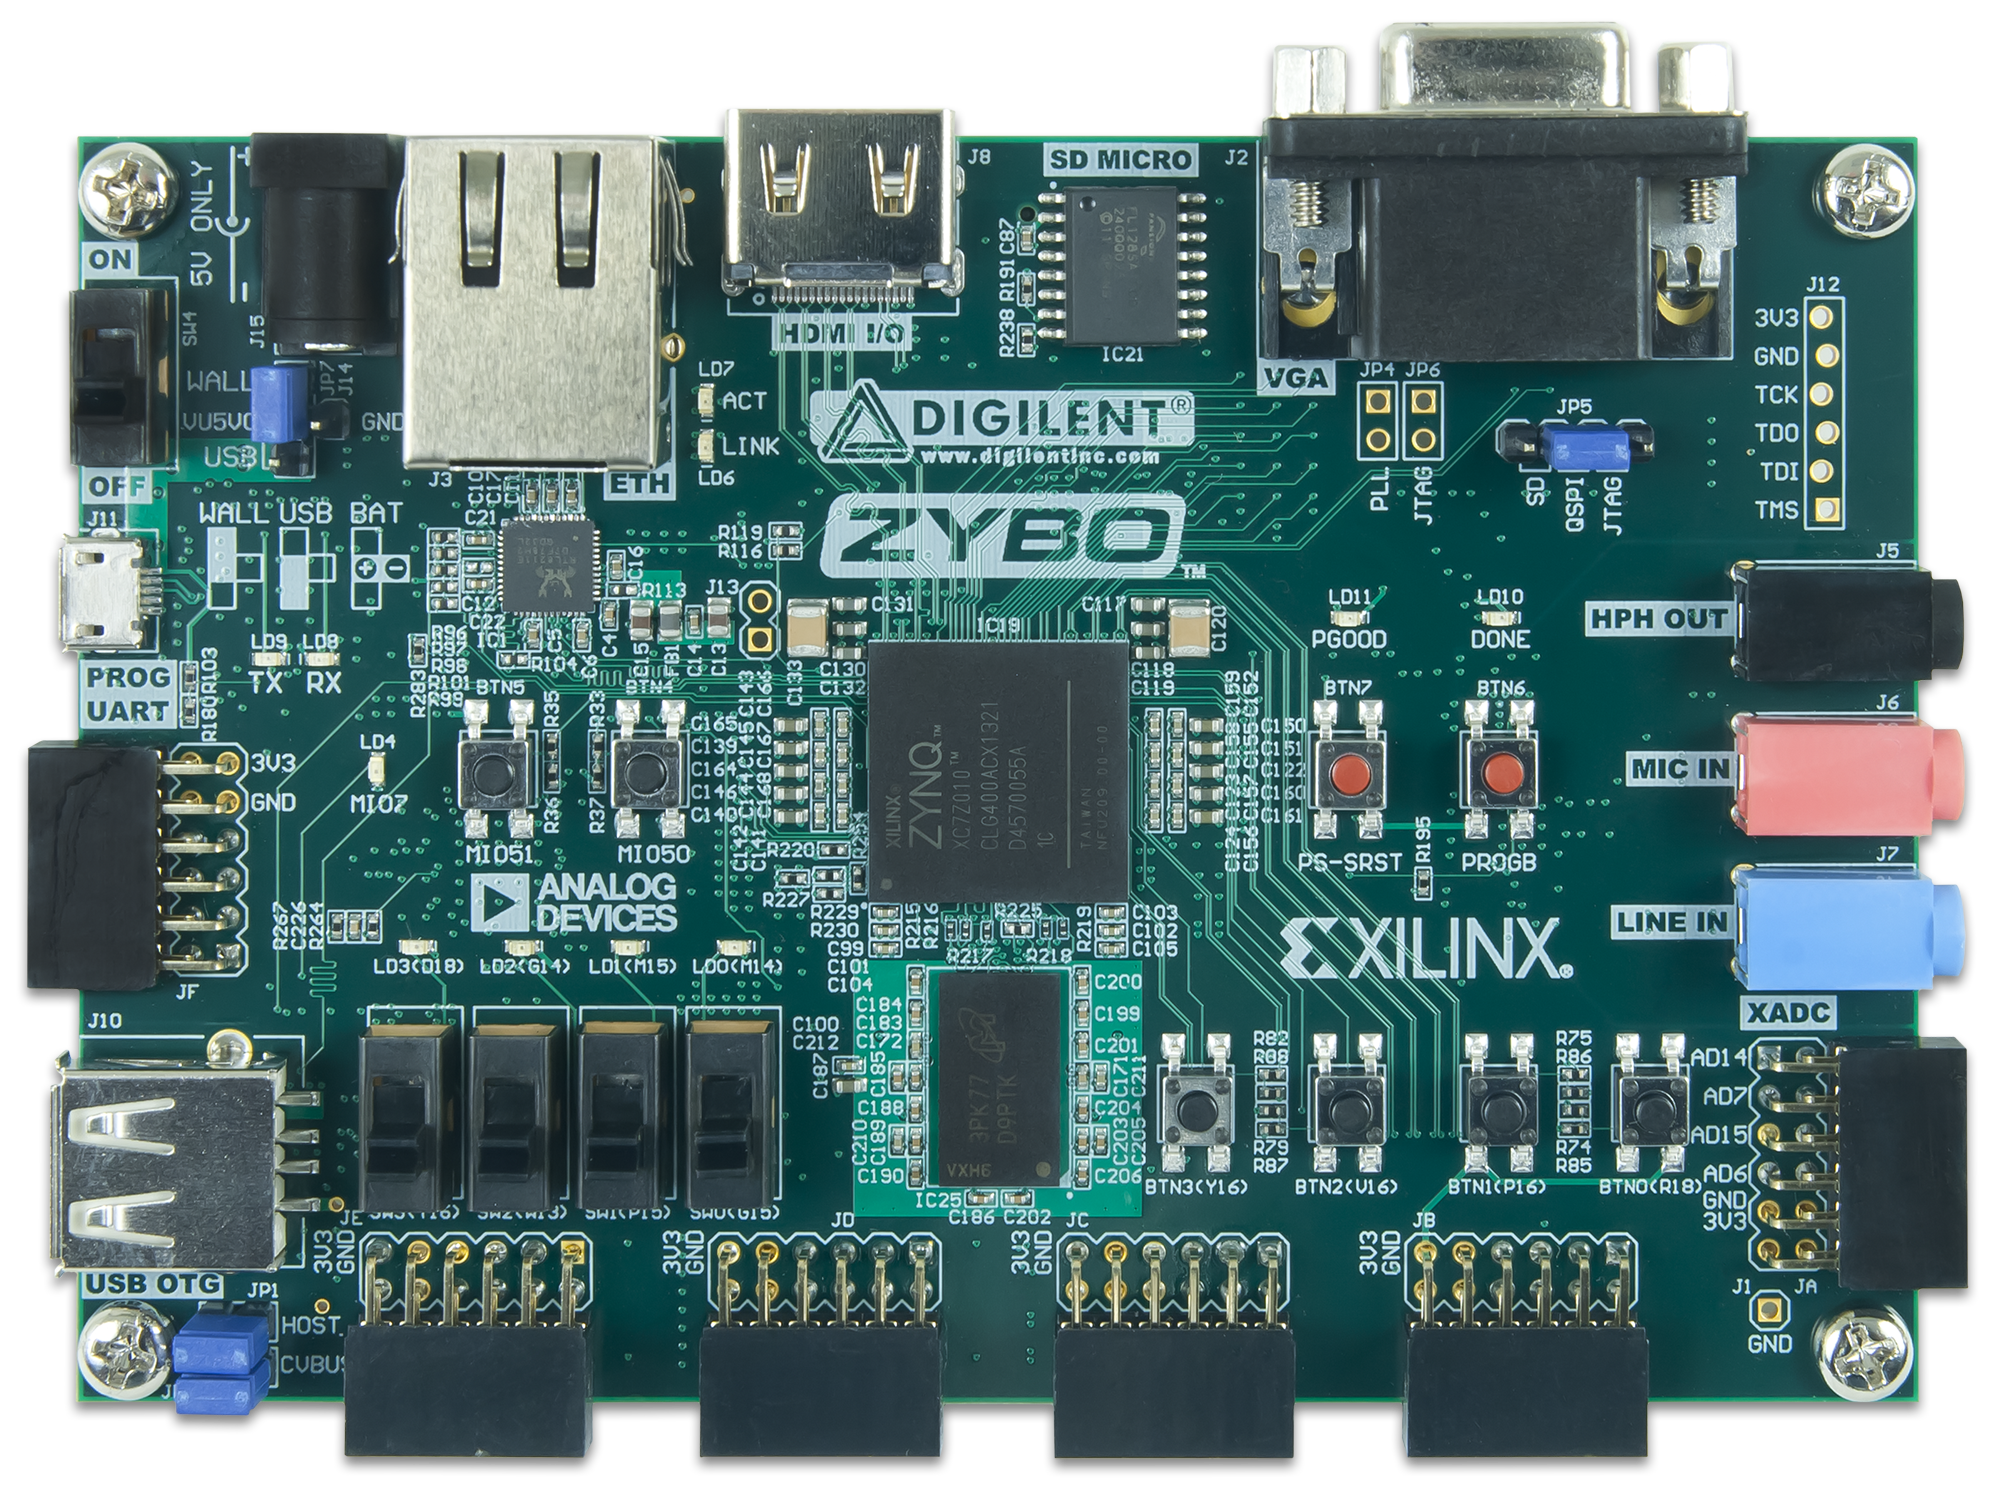
\includegraphics[width = 1\textwidth]{imagenes/zybo.png}
    \caption{ZYBO Zynq-7000 Development Board}\label{zybo}
\end{figure}

Zybo es compatible con \textit{Vivado Design Suite} de Xilinx así como con el conjunto de herramientas ISE/EDK.
Estas herramientas combinan el diseño lógico FPGA con el desarrollo software de ARM en un flujo de diseño intuitivo.
Se pueden utilizar para diseñar sistemas de cualquier complejidad, desde un sistema operativo completo hasta un programa 
simple que controla algunos LEDs.

\textbf{Vivado Design Suite} es un entorno de diseño integrado (\textbf{IDE}) de Xilinx para la síntesis y análisis de diseños HDL. Vivado incluye 
el simulador lógico \textbf{ISim} (\textit{ISE simulator}). Además incluye síntesis a alto nivel con una herramienta que convierte 
código C a lógica programable.

Está formado por 4 componentes\cite{vivado_wiki}:
\begin{itemize}
    \item \textbf{Vivado High-Level Synthesis} - Permite usar programas en \(C\), \(C++\) y \(SystemC\) en dispositivos Xilinx  sin necesidad 
    de crear un RTL manualmente. Aumenta la productividad del desarrollador y admite clases, plantillas, funciones y sobrecarga de operadores.
    \item \textbf{Vivado Simulator} - Es un simulador de lenguaje compilado que admite scripts TCL (\textit{Tool Command Language}) en lenguaje mixto.
    \item \textbf{Vivavo IP Integrator} - Permite integrar y  configurar IP desde la biblioteca propia de Xilinx.
    \item \textbf{Vivado TCL Store} - Es un sistema de comandos para desarrollar complementos para Vivado además de agregar y modificar las 
    capacidades de Vivado. Todas las funciones de Vivado se pueden controlar con los scripts TCL.
\end{itemize}

Para trabajar con Vivado, se puede hacer tanto trabajando con la TCL o directamente con la GUI de Vivado IDE \cite{vivadoIDE}. 
\begin{figure}[H]
    \centering
    \includegraphics[width = 1\textwidth]{imagenes/Vivado1.png}
    \caption{Vivado IDE}\label{vivadoGUI}
\end{figure}

La sección \textbf{Quick Start} nos proporciona fácil acceso a la creación de un nuevo proyecto, abrir proyectos existentes o abrir proyectos 
de ejemplo ofrecidos por Xilinx. Además, en la sección \textbf{Recent Projects} se pueden abrir proyectos usados recientemente.

En la sección \textbf{Tasks} encontramos el acceso a \textbf{Manage IP} que nos permite crear una ubicación IP  para configurar y administrar 
IPs de forma remota. Se puede usar el catálogo de IP de Vivado para personalizar la IP. \textbf{Open Hardware Manager} nos ayuda a programar 
el diseño en el dispositivo. \textbf{Xilinx TCL Store} es un repositorio de código TCL. Da acceso a múltiples scripts para resolver problemas y 
mejorar la productividad.

La última sección es \textbf{Information Centre} donde se encuentra el acceso directo a la documentación, tutoriales y videos sobre lo que se 
puede hacer con esta herramienta.

Los componentes principales de la imagen \ref{vivado2} son:
\begin{enumerate}
    \item \textit{Menu Bar} \ref{menubar}
    \item \textit{Main Toolbar} \ref{maintoolbar}
    \item \textit{Flow Navigator} \ref{flownavigator}
    \item \textit{Layout Selector} \ref{Layoutselector}
    \item \textit{Data Windows Area} \ref{data}
    \item \textit{Workspace} \ref{workspace}
    \item \textit{Menu Command Search Field} \ref{mcsf}
    \item \textit{Project Status Bar} \ref{psb}
    \item \textit{Results Windows Area} \ref{status}
\end{enumerate}

\begin{figure}[H]
    \centering
    \includegraphics[width = 1\textwidth]{imagenes/vivado2.png}
    \caption{Entorno Principal Vivado IDE}\label{vivado2}
\end{figure}

\textit{Menu Bar} nos da acceso a los comandos de Vivado IDE. Normalmente, cuando se inicia un proyecto, no todos los comandos están 
disponibles, sino que algunos se muestran cuando el diseño está activo.

\begin{figure}[H]
    \centering
    \includegraphics[width = 0.7\textwidth]{imagenes/menubar.png}
    \caption{\textit{Menu Bar}}\label{menubar}
\end{figure}

\textit{Menu Command Search Field} se encuentra a la derecha del anterior y permite localizar y ejecutar un comando de manera más rápida. La 
lista de comandos que aparecen en la búsqueda están basados en el contexto del proyecto del diseño actual.

\begin{figure}[H]
    \centering
    \includegraphics[width = 0.5\textwidth]{imagenes/mcsf.png}
    \caption{\textit{Menu Command Search Field}}\label{mcsf}
\end{figure}

\textit{Main Toolbar} nos da acceso a los comandos más usados en Vivado IDE. Si se pone el cursor en alguno de estos comandos, Vivado 
ofrece más información acerca del mismo.

\begin{figure}[H]
    \centering
    \includegraphics[width = 1\textwidth]{imagenes/maintoolbar.png}
    \caption{\textit{Main Toolbar}}\label{maintoolbar}
\end{figure}

\textit{Flow Navigator} permite acceder a comandos y herramientas que van desde abrir diseños a crear un archivo bitstream. Las 
diferentes secciones permiten hacer lo siguiente:
\begin{itemize}
    \item \textit{\textbf{Project Manager}}: Cambio de ajustes generales, añadir o crear archivos o abrir el Catálogo de IPs
    \item \textit{\textbf{IP Integrator}}: Crear, abrir o generar un bloque de diseño. 
    \item \textit{\textbf{Simulation}}: Cambio de ajustes de simulación o simular un diseño activo.
    \item \textit{\textbf{RTL Analysis}}: Abrir un diseño elaborado o generar un diseño de diagrama de circuitos RTL.
    \item \textit{\textbf{Synthesis}}: Cambio de ajustes de síntesis, sintetizar un diseño activo o abrir el diseño sintetizado.
    \item \textit{\textbf{Implementation}}: Cambio de ajuste de implementación, implementar un disñeo activo o abrir el diseño implementado.
    \item \textit{\textbf{Program and Debug}}: Cambio de ajustes del bitstream, generar un archivo bitstream o abrir una sesión hardware.
\end{itemize}

\begin{figure}[H]
    \centering
    \includegraphics[width = 0.5\textwidth]{imagenes/flownavigator.png}
    \caption{\textit{Flow Navigator}}\label{flownavigator}
\end{figure}

\textit{Layout Selector} proporciona el diseño de ventanas predefinidas para facilitar el proceso de diseño. Entre las opciones tenemos:
\begin{itemize}
    \item \textit{\textbf{Default Layout}}: Analización del diseño con el mínimo número de ventanas
    \item \textit{\textbf{I/O Planning}}: Definición de restricciones de ubicación I/O y colocación de puertos.
    \item \textit{\textbf{Clock Planning}}: Planificación y colocación de los recursos del reloj del diseño.
    \item \textit{\textbf{Floorplanning}}: Gestionar particiones y tareas jerárquicas.
    \item \textit{\textbf{Timing Analysis}}: Ejecutar informes de tiempo y analizarlo.
\end{itemize} 

\begin{figure}[H]
    \centering
    \includegraphics[width = 0.5\textwidth]{imagenes/Layoutselector.png}
    \caption{\textit{Layout Selector}}\label{Layoutselector}
\end{figure}

\textit{Project Status Bar} da información sobre el estado actual del diseño activo.

\begin{figure}[H]
    \centering
    \includegraphics[width = 0.3\textwidth]{imagenes/psb.png}
    \caption{\textit{Project Status Bar}}\label{psb}
\end{figure}

\textit{Data Windows Area} muestra información sobre los archivos que forman el diseño.

\begin{figure}[H]
    \centering
    \includegraphics[width = 0.7\textwidth]{imagenes/datawa.png}
    \caption{\textit{Data Windows Area}}\label{data}
\end{figure}

\textit{Workspace} muestra ventanas como el editor de textos o el diseño del diagrama de circuitos, entre otros.

\begin{figure}[H]
    \centering
    \includegraphics[width = 0.7\textwidth]{imagenes/workspace.png}
    \caption{\textit{Workspace}}\label{workspace}
\end{figure}

\textit{Results Windows Area} presenta los resultados de los comando ejecutados. Además se muestran distintas ventanas, como 
\textit{Tcl Console}, \textit{Messages}, \textit{Log}, \textit{Reports} y \textit{Design Runs}.

\begin{figure}[H]
    \centering
    \includegraphics[width = 1\textwidth]{imagenes/statusbar.png}
    \caption{\textit{Results Windows Area}}\label{status}
\end{figure}

\section{Metodología}

\section{Desarrollo de módulos hardware específicos}

\section{Casos prácticos}


\chapter{Conclusiones y vías futuras}

Como resultado, se han conseguido los objetivos marcados, se ha conocido y estudiado una plataforma de carácter didáctico, Vivado, a partir de la documentación facilitada 
por el fabricante Xilinx, para la realización de ejercicos prácticos que sean útiles para el aprendizaje del diseño de sistemas basados en FPGAs a partir de descripciones VHDL para síntesis RT. 

Xilinx es la empresa líder en la fabricación de FPGAs además de en herramientas de desarrollo en los distintos niveles de síntesis automática. Además se 
ha analizado la plataforma Vivado junto con la tarjeta Zybo para el estudio de la metodología y flujo de diseño de sistemas basados en FPGAs a partir de descripciones VHDL para síntesis RT.

Se ha realizado un ejemplo sencillo (contador de 4 bits) con el que se ha validado el flujo de diseño y después se han realizado un par de ejemplos prácticos, un computador 
básico y la visualización de una bola en la pantalla, validando módulos VHDL útiles en las prácticas de laboratorio de la asignatura ``Desarrollo de Hardware Digital'', como un porcesador y 
un controlador VGA. Además para la realización de estos ejemplos se ha tenido que generar módulos de memoria y de generación de reloj a partir del catálogo de componentes 
IP de Vivado, los cuales se han validado y se ha comprobado su correcto funcionamiento.

Es cierto que al principio hubo algunos problemas con respecto a conocer la tarjeta usada y la plataforma de desarrollo, además de con la realización 
de los ejemplos prácticos. Todo esto ha tenido un buen resultado, por lo que se puede decir que se han cumplido los objetivos de este trabajo de fin de grado, resultando viable 
y satisfactoria la migración de las prácticas de la asignatura DHD para su realzación con la herramienta Vivado y con la tarjeta de desarrollo Zybo.

Como posibles vías futuras se puede considerar la ampliación del número de módulos VHDL para integración de sistemas de interés pedagógico como módulos de interfaz PS/2 para teclado y 
ratón o módulos sencillos de comunicaciones como I2C o UART. Otra podría ser ampliar la plataforma con módulos descritos en C/C++ útiles en asignaturas de perfil más 
avanzado que emplean Vivado HLS. Incluso se podría utilizar otra tarjeta de caracter didáctico como la Zybo Z7 que es la versión actualizada de la Zybo.

La herramienta Vivado se emplea en algunas asignaturas del Máster en el que me he matriculado. Este Máster proporciona una visión general del estado del arte de las 
actuales y futuras tecnologías electrónicas, así como una base específica y metodológica para poder realizar labores de investigación y desarrollo en el área de los 
sistemas electrónicos.

Algunas de las asignaturas de este máster contienen entre otros temas la arquitectura interna de las FPGAs así como las tecnologías de fabricación más modernas y los 
principales fabricantes de estas. También se usa la herramienta Vivado usada en este trabajo para realizar prácticas con una placa de Digilent que incluye una 
FPGA Artix-7 de Xilinx. 

\clearpage
\nocite{*}
\bibliographystyle{plain}
\bibliography{bibliografia/bibliografia}

%Se incluirá tanto las fuentes primarias como todas aquellas cuyo peso haya sido menor en la realización del trabajo. Un breve comentario de las referencias es conveniente, que puede ser individualizado, por grupos de referencias o global.
%En caso de incluir URLs de páginas web (se recomienda no abusar de ellas), éstas deben ser acompañadas de título, autor, fecha de último acceso, entre otros datos relevantes.

\end{document}
